A rectangle has sides of length $a$ and $36$. A hinge is installed at each vertex of the rectangle and at the midpoint of each side of length $36$. The sides of length $a$ can be pressed toward each other keeping those two sides parallel so the rectangle becomes a convex hexagon as shown. When the figure is a hexagon with the sides of length $a$ parallel and separated by a distance of $24,$ the hexagon has the same area as the original rectangle. Find $a^2$.


\begin{center}
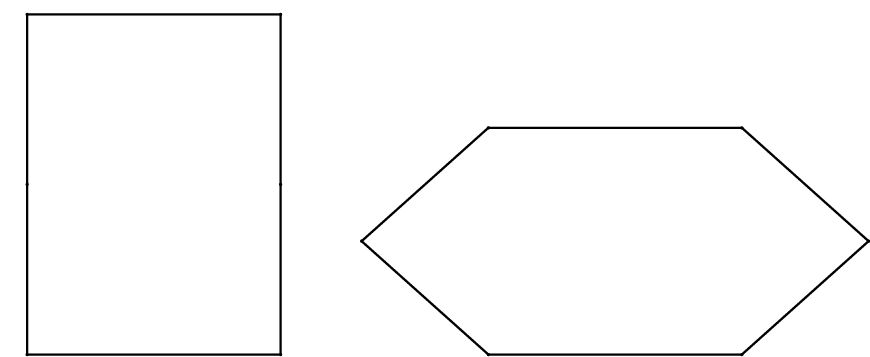
\includegraphics[width = 87.0mm]{img/fig0.png}
\end{center}